\subsection{Библиотека Джона Хьюза}

Библиотека Джона Хьюза, описанная в \cite{hughes}, явялется первой комбинаторной pretty printing библиотекой. Она основана на алгоритме, предложенном Дереком Оппеном в \cite{oppen}, по сути является его реализацией в функциональном стиле на Haskell. Также библиотека Джона Хьюза, расширенная Саймоном Пейтоном Джонсом \cite{peytonJones}, является стандартной pretty print библиотекой для Haskell.

% рассказать об оптимальном

В данной библиотеке ключевым типом является \textbf{Doc}. Основные комбинаторы для составления документа:
\inputminted{haskell}{codes/hughesBasicOperators.hs}

Так с помощью функции \textbf{text} по строке получается документ, оператор \textbf{(<>)} соединяет два документа горизонтально (см. рисунок~\ref{fig:hughesHorComp}), а оператор \textbf{(\$\$)} соединяет документы вертикально (см. рисунок~\ref{fig:hughesVertComp}).

\begin{figure}[h!]
	\begin{minipage}[b]{0.45\linewidth}
		\centering
		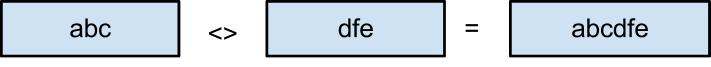
\includegraphics[width=\textwidth]{hughesHorComp}
		\caption{}
		\label{fig:hughesHorComp}
	\end{minipage}
	\hspace{0.5cm}
	\begin{minipage}[b]{0.45\linewidth}
		\centering
		
\includegraphics[width=\textwidth]{hughesVertComp}
		\caption{}
		\label{fig:hughesVertComp}
	\end{minipage}
\end{figure}

В обычном случае функция \textbf{nest} добавляет к каждой строке заданное число ведущих пробелов. Но в комбинации с функцией \textbf{sep}, может вообще не поменять документ.

Функция \textbf{sep} является ключевым комбинатором, который в этой библиотеке позволяет задавать плавающую раскладку документа. Она принимает как параметр список документов, а на выходе получается документ, который представляет из себя либо вертикальную склейку элементов списка, либо горизонтальную склейку (как раз в этом случае функция \textbf{nest} не изменяет документ), причем между документами вставляется пробельный символ. Вариант раскладки выбирается функцией \textbf{pretty}:

\inputminted{haskell}{codes/hughesPretty.hs}

Кроме самого документа, функция \textbf{pretty} также принимает два числа: максимальную длину и максимальную наполненность строки. Здесь наполненность строки значит длину текста без ведущих пробельных символов. В ходе работы этой функции и происходит выбор раскладки документа, полученного с помощью комбинатора \textbf{sep}. Если горизонтальная раскладка удовлетворяет ограничениям на ширину строки, то она и выбирается. Иначе -- вертикальная раскладка.


% Возможно, стоит сделать после обзора всех библиотек

Рассмотрим пример описания pretty printer с помощью библиотеки Хьюза. Для этого используем учебный язык L. Он состоит из небольшого числа операторов:
\begin{enumerate}
\item присваивание;
\item While;
\item If
\item последовательное выполнение;
\item чтение с занесение в переменную;
\item печать целочисленного выражения.
\end{enumerate}

На рисунке~\ref{fig:lEx} приведен пример программы на языке L. В данном случае, это программа, которая считывает с консоли два числа, а потом возводит второе число в степень, равную первому.

\begin{figure}[h!]
	\centering
	\inputminted{pascal}{codes/lEx.l}
	\caption{Быстрое возведение в степень на L}
	\label{fig:lEx}
\end{figure}

Часть pretty printer
\footnote{В примере используется неописанный выше комбинатор \textbf{(<+>)}. Это просто сокращение записи. \textit{a <+> b = a <> (text << >>) <> b}. }
для языка L, отвечающая за представление операторов, показана на рисунке~\ref{fig:lHughesPrinter}.
\begin{figure}[h!]
	\inputminted{haskell}{codes/lHughesPrinter.hs}
	\caption{Pretty printer, написанный с помощью библиотеки Хьюза}
	\label{fig:lHughesPrinter}
\end{figure}

В данном случае pretty printer получился несложным, но абсолютно ненаглядным. Также поскольку в библиотеке нет механизмов, позволяющих явно варьировать раскладку документа в зависимости от раскладки его поддокументов, то невозможно выразить пример с рисунка~\ref{fig:lGoodWriteEx}. То есть, если выражение в операторе \textit{write} занимает несколько строк, то закрывающую скобку напечатать на новой строке, на уровне самого оператора.
\begin{figure}[h!]
	\inputminted{pascal}{codes/lGoodWriteEx.l}
	\caption{Желательный пример печати конструкции \textbf{Write}}
	\label{fig:lGoodWriteEx}
\end{figure}

С помощью реализации pretty printer с рисунка~\ref{fig:lHughesPrinter}, в данном случае для оператора \textit{write} получится немного не то (см. рисунок~\ref{fig:lCurWriteEx}).
\begin{figure}[h!]
	\inputminted{pascal}{codes/lCurWriteEx.l}
	\caption{Результат для текущего pretty printer}
	\label{fig:lCurWriteEx}
\end{figure}

А если попробовать поменять функцию \textbf{docFromOperation} для конструкции \textit{Write} (см рисунок~\ref{fig:lHughesWriteChange}), то получится то, что надо в случае если выражение занимает насколько строчек, но в случае с одной строчкой -- перед закрывающей скобкой лишний пробел.
\begin{figure}[h!]
	\inputminted{pascal}{codes/lBadWriteEx.l}
	\caption{Результат для измененого pretty printer}
	\label{fig:lBadWriteEx}
\end{figure}

\begin{figure}[h!]
	\inputminted{haskell}{codes/lHughesWriteChange.hs}
	\caption{}
	\label{fig:lHughesWriteChange}
\end{figure}